\chapter{Loop Closures using an Omni Camera}
\label{chapter:omni_loop_close}

\section{Place Recognition}

The first step is to substitute omni camera images in the place recognition module. The donut image format is not preferred for the place recognition.  They contains blind spots (inner and outer circle), which contain some texture, and are also susceptible to change from internal reflections within the lense.  In terms of place recognition, this would add noise to each image and therefore the unwrapped image is preferred.

It is computational expensive to unwrap every frame, this would mean processing 1280x960 images at 30Hz.  This would also introduce complications in synchronizing stereo frames with omni frames.  Therefore only keyframe images are unwrapped.  A omni camera image buffer records a short history of donut image frames.  When a new keyframe is created, the timestamp of the stereo image used for this keyframe is sent to the buffer object, which finds the corresponding omni camera image and unwraps it.  This unwrapped image is saved with the keyframe and sent to the place recognition module.  This reduces computational cost and simplifies omni-stereo synchronization.

As described in section \ref{sec:bag_of_words}, the place recognition system employs clustering of detected SURF features in feature space using a bag of words approach.  This means that in the case of $360^\circ$ circular images, it will be invariant to rotation about the upward facing axis, as the locations of 2D features are not considered.  This is ideal for this particular use case.

\section{Calculating transformations for loop closures}

A match from the place recognition module itself is not enough to do a global loop closure.  As described in section \ref{sec:scavislam_place_recog}, a geometry check is required to filter false positive matches and determine a metric rigid body transformation so the loop closure may be added to the graph.

It has also been mentioned in section \ref{subsec:selected_approach} that calculating a transformation using a monocular camera such as the omni camera introduces the arbitrary scale issue.  (For further explanation of the scale issue, see Chapter \ref{chapter:MultiCamSLAM}). Therefore the stereo information needs to be combined with the omni camera in order to produce a metric scale transformation.  Two methods were developed to address this scale issue, a 'scale correction' algorithm, and using the p3p algorithm.  These methods will be discussed in detail in the following sections.

\subsection{Scale Correction algorithm}

The main idea behind this algorithm is a two stage approach, first calculate the non-metric transformation using omni data and then correct it to metric scale using stereo data.  Take note that the whole idea of using the omni camera is to find loop closures where stereo wouldn't, and therefore the stereo frames will often not be overlapping.

\subsubsection{Pose estimation}

First step is to calculate a non metric transformation using the two omni frames only.  This is done using the 5 point algorithm as mentioned in section \ref{subsec:5point}.  This returns a non metric pose and a set of inlier points used to calculate this pose, represented as 3D vectors (also non metric scale).

\subsubsection{Scale Offset Calculation}

Points with metric scale are calculated using stereo matching.  These points are then matched and compared to 3D points returned from the pose estimation.  A scale offset is calculated per point.  The algorithm that calculates a vector of scale offsets is detailed below.  This algorithm takes as left, right and omni images as an input, and may be applied to either of the two loop closure frames separately.  In practice both are performed and the scale vectors concatenated. 

\begin{enumerate}
\itemsep0em
 \item Perform circular matching between left/right/omni images %TODO screenshot
 \item Triangulate 3D points in metric scale using left/right stereo circular matches
 \item For each 3D stereo point:
 \begin{enumerate}
   \item Ensure the matching omni point was used in pose estimation
   \item Obtain the 3D non metric point used in pose estimation
   \item Transform the stereo point to the omni cam frame %$(\bv P_{om} =  ^{om}\bv T_{st} \bv P_{st})$
   \item Calculate scale offset as per formula \ref{eq:scale_offset} %TODO
   \item Add to list of offsets 
 \end{enumerate}
\end{enumerate}

\begin{figure}[H]
  \centering
    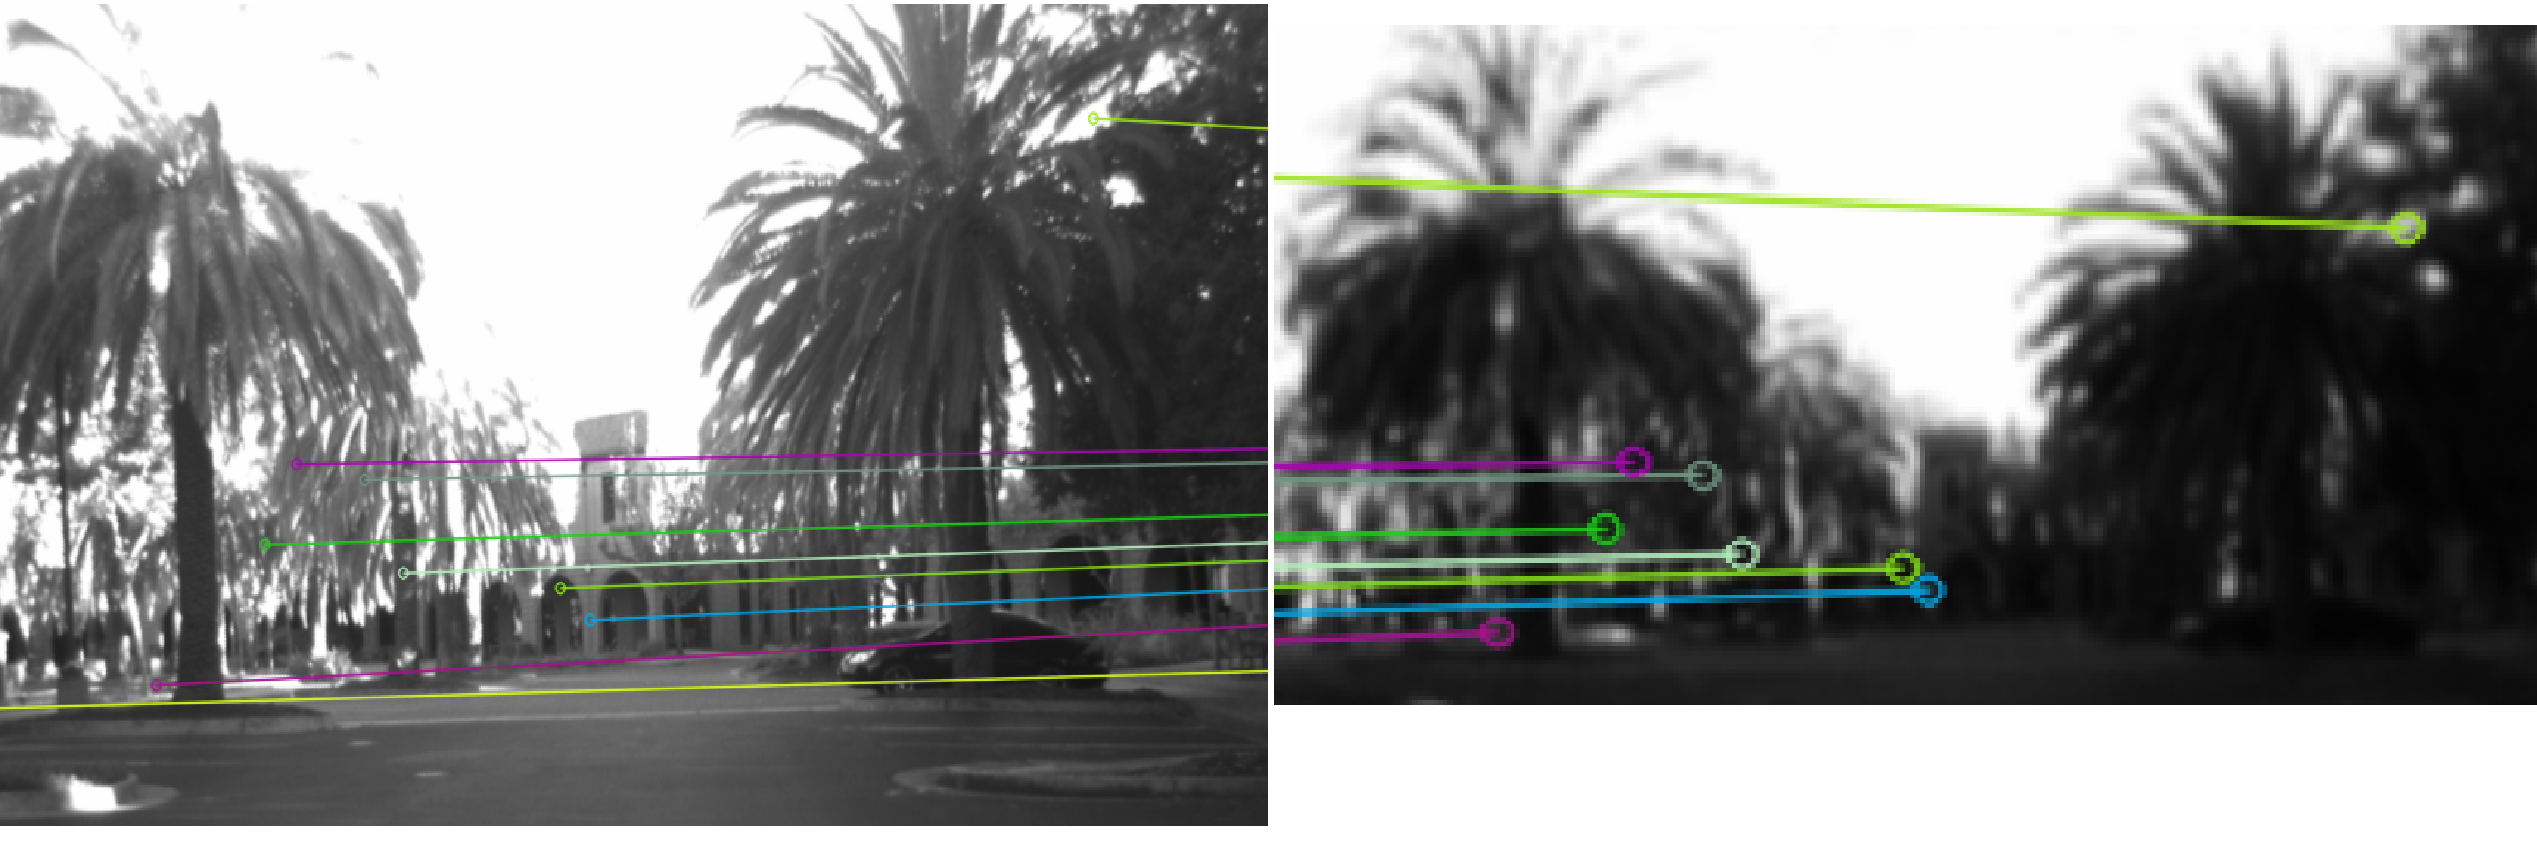
\includegraphics[width=1.0\textwidth]{chapters/images/circular_match}\\
  \caption{Results of circular matching between left, right and omni frames. Left is one of the stereo images and right is a cropped part of the unwrapped omni image. The circular matching produces robust matches without having strict SIFT matching thresholds}
  \label{fig:circular_match}
\end{figure}

\begin{figure}[h]
  \centering
  \begin{align}
   S =
   \displaystyle\frac{
   \left|\displaystyle\frac{\bv {MP}_{x}}{\bv P_{x}}\right| + 
   \left|\displaystyle\frac{\bv {MP}_{y}}{\bv P_{y}}\right| + 
   \left|\displaystyle\frac{\bv {MP}_{z}}{\bv P_{z}}\right|
   }
   {3}
  \end{align}
  \caption{Scale calculation for a single point.  $\bv{MP}$ denotes the metric 3D point calculated from stereo and $\bv{P}$ denotes the non metric 3D point used in pose estimation}
  \label{eq:scale_offset}
\end{figure}

%TODO visualization of scale offsets

%TODO visualization of 180 deg pose: slides from last intern meeting

\subsubsection{Robust scale estimation}

Having determined a number of scale offsets, a single offset needs to be determined.  It is likely that outliers exist in the data and need to be considered.  A potential approach would be to apply RANSAC, choosing a single point and scaling the values and comparing them to their correspondences.  A simpler and less computationally expensive method would be to calculate a robust mean.  A robust mean is calculated in this case using some guys robust mean algorithm (citation).

%TODO robust mean citation

\begin{figure}[H]
  \centering
    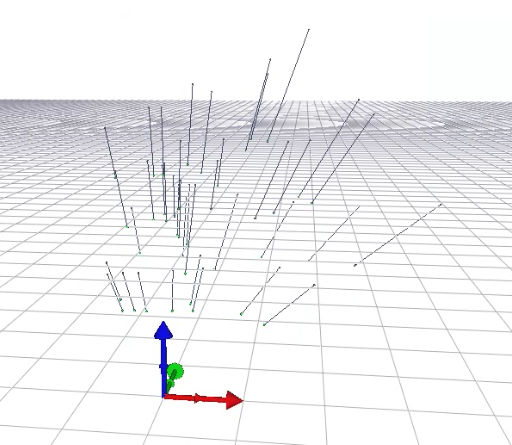
\includegraphics[width=0.7\textwidth]{chapters/images/scale_matches}\\
  \caption{Visualization of non metric points and their corresponding metric scale matches}
  \label{fig:circular_match}
\end{figure}

\subsection{p3p Implementation}

As opposed to the two step approach described above, this implementation calculates a metric transformation using stereo and omni data in one step.

The p3p algorithm (cite, section \ref{subsec:p3p}) calculates a transformation between frames given a set of 2D to 3D correspondences.  The scale of the transformation is propagated from the 3D points.  This means after triangulating the new 2D points with the transformation obtained, they will be to the same scale as the existing map.

In this case this algorithm could be used the following way:

\begin{enumerate}
\itemsep0em
 \item Perform circular matching between left/right images from one keyframe, and omni image from the other keyframe
 \item Triangulate 3D points in metric scale using left/right stereo circular matches
 \item Use p3p algorithm; correspondences are known between 3D stereo points and 2D omni points
\end{enumerate}

This will directly calculate a pose between the two keyframes to the correct scale.  It can also be run twice, matching stereo and omni in both directions. In terms of implementation this is a much neater solution, and would be preferred.  However there are a few pitfalls why it was not chosen as the solution to evaluate on.

In practice it turns out to be not as accurate.  The number of matches between the stereo camera and the omni camera of the other keyframe is typically very low.  Whilst in the scale correction algorithm, these matches are only used for scale adjustment, in this case they are used for pose estimation.  Scale adjustment only requires 1 correspondence, however pose estimation requires 3.  There are likely to be outliers and therefore desirably a factor of the minimal number of correspondences is needed to determine a good pose.

Another advantage of the scale adjustment algorithm is the way in which the data from both frames is fused.  For both algorithms, they can be run twice using first one keyframe, and then the other.  Whilst the scale adjustment algorithm outputs two offset vectors that can easily be combined to determine a robust mean, the p3p implementation generates two separate poses that need to be fused together somehow.  They could be averaged or both added to the graph weighted on the number of inliers, however one can think of the other algorithm producing a single, higher quality transformation from the same data.
REWRITE THIS CRAP. COPY MATCHING PIC FROM SLIDES
 
\begin{figure}[H]
  \centering
    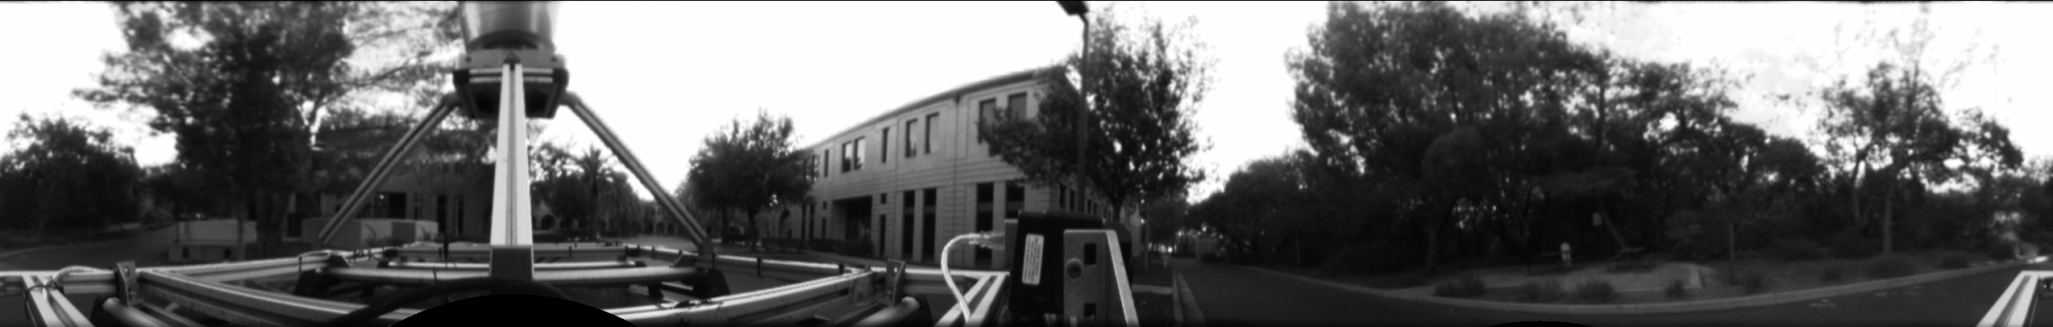
\includegraphics[width=1.0\textwidth]{chapters/images/omni_source}\\
    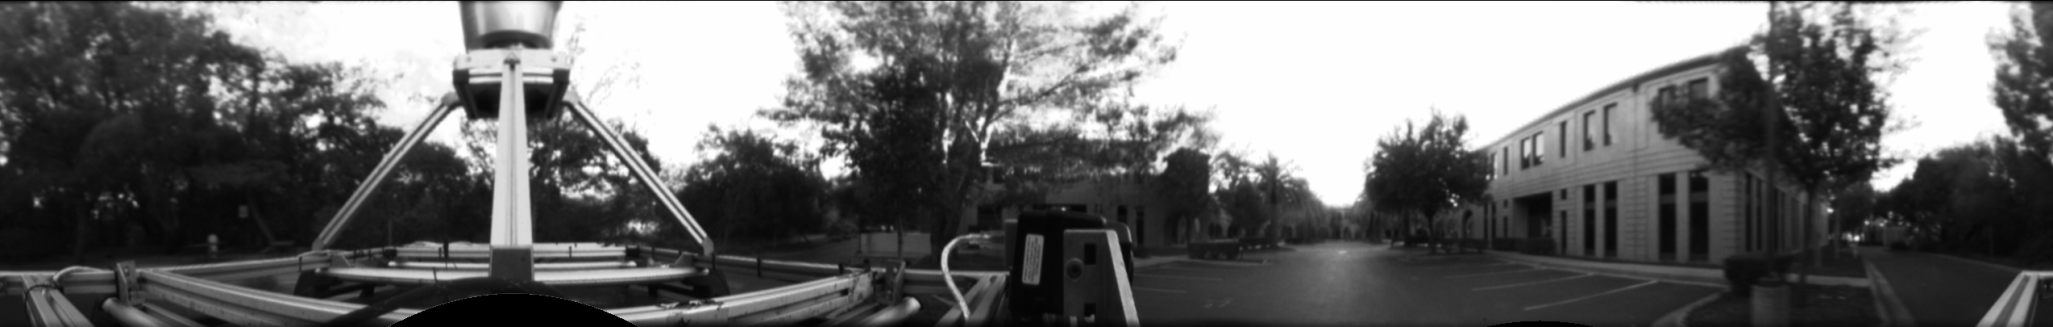
\includegraphics[width=1.0\textwidth]{chapters/images/omni_target}\\
    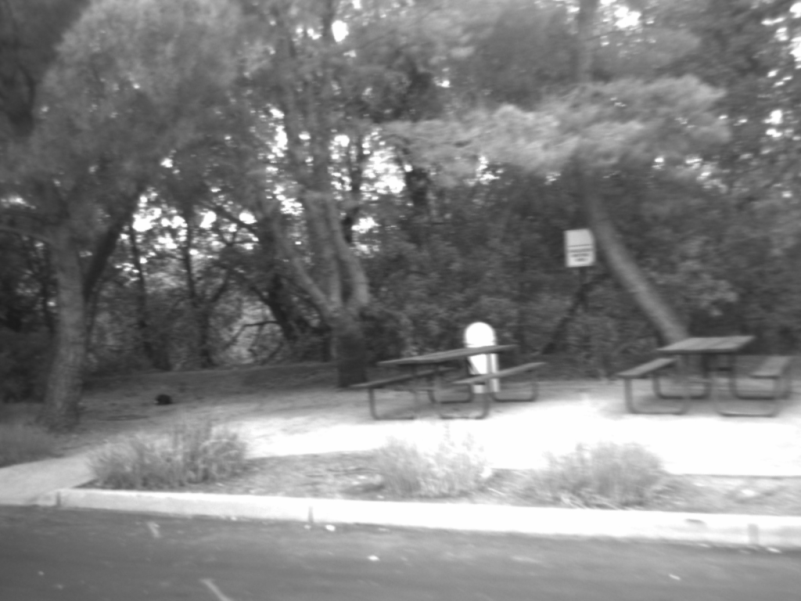
\includegraphics[width=0.49\textwidth]{chapters/images/stereo_source}
    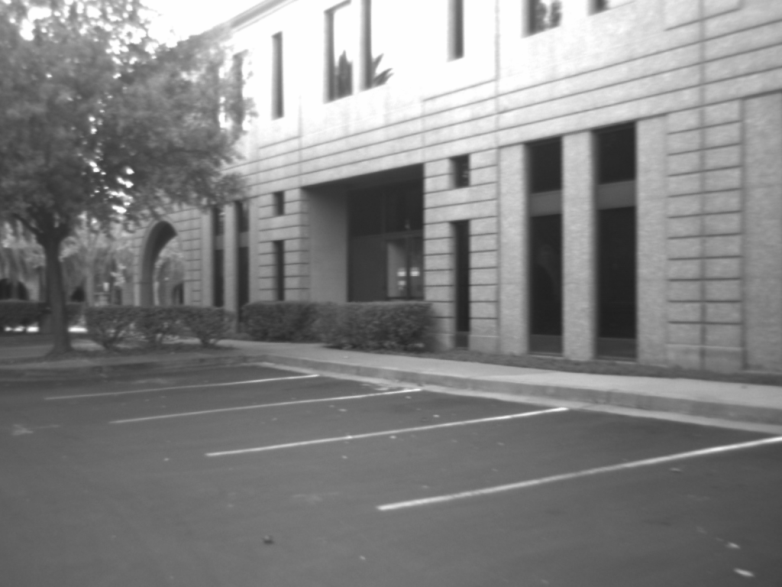
\includegraphics[width=0.49\textwidth]{chapters/images/stereo_target}\\
    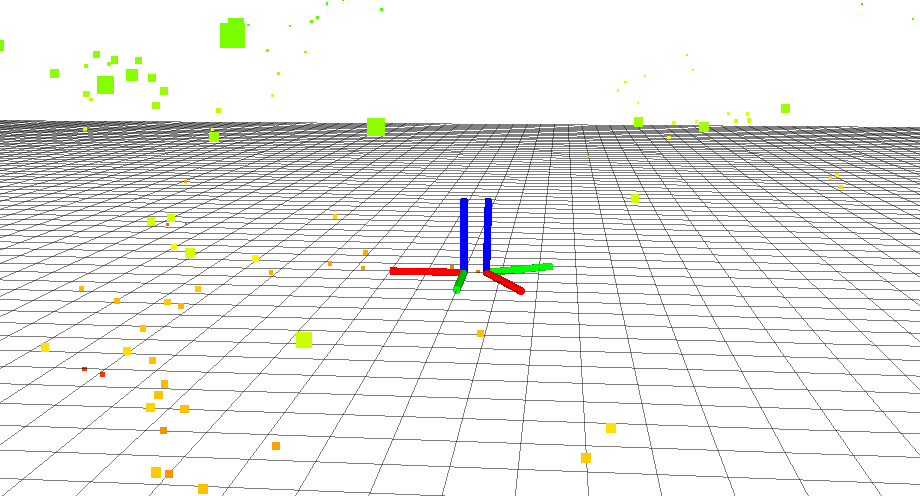
\includegraphics[width=1.0\textwidth]{chapters/images/loop_closure_pose}
  \caption{Example of a pose invariant loop closure using scale adjustment algorithm.  Top shows the two omni images.  Middle shows what the stereo camera sees from these poses.  There is clearly no overlap in the stereo frames.  Bottom shows the metric transformation visualized as a pose, along with 3D pose inlier points in metric scale.}
  \label{fig:}
\end{figure}
\section{Introducing loop closure constraints to the SLAM graph}

\begin{itemize}
\itemsep0em
 \item  double win not trivial
 \item single edge not strong enough - removes one keyframe, doesn't move inner window
 \item frames need to be initialized in new location
 \item edge only optimization to init
 \item restore double window
\end{itemize}